\chapter{Test}

Dopo aver visto questi modelli, possiamo vedere le varie differenze tra di loro andando a confrontarli
con quelle che sono le proprietà principali per la valutazione di un modello, le quali abbiamo visto in precedenza.

\noindent
Per condurre questo studio e avere un solido punto di riferimento esterno, abbiamo inizialmente selezionato un modello di terze parti. Di tale modello non possediamo dettagli specifici riguardanti l'architettura esatta,
la provenienza dei dati originali o le metodologie con cui è stato precedentemente addestrato; operando in assenza di queste informazioni a priori, esso si è configurato per noi, a tutti gli effetti,
come un sistema a "scatola chiusa" (black box).

\section{Ground truth}

\noindent
Per poter valutare oggettivamente le prestazioni di questo strumento e degli altri algoritmi a nostra disposizione, è emersa la necessità fondamentale di definire un metro di giudizio assoluto, rigoroso e imparziale.
A tale scopo, abbiamo costruito una cosiddetta ground truth (verità di base) partendo dal medesimo dataset di immagini che sarebbe stato poi sottoposto in fase di test. Nello specifico,
l'intero set di dati è stato analizzato e verificato manualmente, ispezionando il campione un'immagine alla volta. Questo meticoloso processo di revisione umana ci ha permesso di generare un dataset pulito,
accurato e privo di errori, che rappresenta il risultato ideale a cui ogni algoritmo dovrebbe tendere.

\noindent
La ground truth è composta, per ogni immagine, da un insieme di oggetti annotati manualmente. Ogni oggetto è descritto da:
\begin{itemize}
  \item una \textbf{classe}, scelta dalla tassonomia del dataset;
  \item un \textbf{bounding box}, cioè il rettangolo che racchiude l'oggetto, espresso in pixel tramite le coordinate $(x_1, y_1, x_2, y_2)$ degli angoli opposti.
\end{itemize}

\noindent
La valutazione si concentra sulle tre classi \textit{upper clothing}, \textit{lower clothing} e \textit{footwear}. Il bounding box è quindi l'unità di misura comune:
qualunque sia il tipo di output di un modello, questo viene sempre ricondotto a dei box prima del confronto.

\noindent
Il valore strategico di questa ground truth si è rivelato cruciale per l'intera fase di testing. Essa, infatti, non è servita esclusivamente a valutare il modello black box, ma è stata impiegata come standard universale
per testare e verificare le performance di svariati altri modelli che abbiamo preso in esame.

\noindent
I modelli da confrontare sono molto diversi tra loro (detector, modelli di segmentazione, modelli open-vocabulary e il modello black box), per cui è necessario che le loro predizioni vengano misurate tutte nello stesso modo.
Abbiamo quindi definito un unico protocollo di valutazione, indipendente dall'architettura del singolo modello: ogni modello viene eseguito sulle immagini della ground truth, le sue predizioni vengono ricondotte a un formato comune
e infine confrontate con le annotazioni manuali.

\subsection{Abbinamento tra predizioni e ground truth}

\noindent
Il passaggio centrale della valutazione è decidere quale predizione corrisponde a quale oggetto della ground truth. Per ogni immagine l'abbinamento avviene in modo \textit{greedy}:
\begin{enumerate}
  \item le predizioni vengono ordinate dalla più confidente alla meno confidente;
  \item per ogni predizione, in quest'ordine, si cerca tra gli oggetti della ground truth non ancora assegnati quello con il punteggio di sovrapposizione più alto;
  \item se questo punteggio supera la soglia prevista, la predizione e l'oggetto vengono abbinati e l'oggetto non può più essere assegnato ad altre predizioni;
        altrimenti la predizione resta senza abbinamento.
\end{enumerate}

\noindent
Ogni oggetto della ground truth può quindi essere abbinato a una sola predizione, e se un modello produce più box sullo stesso oggetto, solo il più confidente viene abbinato, mentre gli altri vengono considerati errori.
Da notare che il punteggio di sovrapposizione usato per l'abbinamento cambia a seconda del tipo di modello.

\newpage

\paragraph{Detection}
Per i modelli di detection si usa l'IoU, che come abbiamo visto misura quanto il box predetto $P$ e il box della ground truth $G$ coincidono.

\paragraph{Segmentazione}
Per i modelli di segmentazione l'IoU risulterebbe troppo severo, visto che il box ricavato da una maschera può essere più piccolo del box annotato, ad esempio quando una parte del capo è coperta,
oppure quando la maschera lo segue più da vicino del rettangolo disegnato a mano. In questi casi l'oggetto è stato trovato, ma l'IoU sarebbe basso.
Per questo motivo si usa il \texttt{contenimento}, che misura quanta parte della predizione cade all'interno del box della ground truth:
$$ \mathrm{C}(P, G) = \frac{|P \cap G|}{|P|} $$

\noindent
Il contenimento vale 1 quando la predizione è interamente contenuta nell'oggetto annotato, senza pretendere che ne indovini l'esatta estensione. Poiché anche un box minuscolo interno all'oggetto avrebbe contenimento pari a 1,
si aggiunge un controllo sulla copertura, cioè sulla parte del box della ground truth coperta dalla predizione:
$$ \mathrm{Cov}(P, G) = \frac{|P \cap G|}{|G|} $$

\noindent
Una predizione viene abbinata se $\mathrm{C} \geq 0.5$ e $\mathrm{Cov} \geq 0.1$. \\

\begin{figure}[htbp]
  \centering
  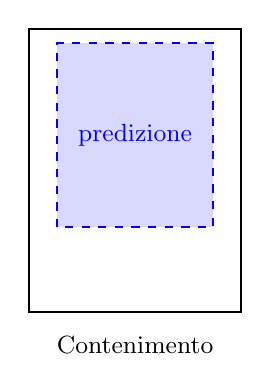
\begin{tikzpicture}[scale=0.9]
    % Esempio contenimento: box predetto più piccolo, dentro la GT
    \draw[thick, black] (8,0) rectangle (11,4);
    \draw[thick, dashed, blue] (8.4,1.2) rectangle (10.6,3.8);
    \fill[blue, opacity=0.15] (8.4,1.2) rectangle (10.6,3.8);
    \node[blue] at (9.5,2.5) {\small predizione};
    \node[below] at (9.5,-0.2) {\small Contenimento};
  \end{tikzpicture}
  \caption{Una predizione interamente contenuta nell'oggetto}
  \label{fig:iou_contenimento}
\end{figure}

\newpage

\subsection{Confusion matrix}

\noindent
Una volta abbinate le predizioni, i risultati di tutte le immagini vengono raccolti in una confusion matrix. In questa fase si considerano solo le predizioni con confidenza di almeno $0.5$, così da valutare il modello nelle condizioni
in cui verrebbe realmente usato.

\noindent
Le righe della matrice rappresentano la classe reale (quella della ground truth), le colonne la classe predetta. Oltre alle classi, la matrice contiene:
\begin{itemize}
  \item una riga \texttt{background}, per le predizioni che non sono state abbinate a nessun oggetto (il modello ha visto un oggetto dove non c'era);
  \item una colonna \texttt{background}, per gli oggetti della ground truth rimasti senza predizione (il modello non li ha visti);
  \item una colonna \texttt{non mappate}, per le predizioni con una classe estranea alla ground truth.
\end{itemize}

\begin{table}[htbp]
  \centering
  \renewcommand{\arraystretch}{1.3}
  \begin{tabular}{lcccc}
    \toprule
    \textbf{GT $\backslash$ Pred} & \textbf{upper} & \textbf{lower} & \textbf{footwear} & \textbf{background} \\
    \midrule
    \textbf{upper}      & \textbf{TP} & - & -- & FN \\
    \textbf{lower}      & -- & \textbf{TP} & -- & FN \\
    \textbf{footwear}   & -- & -- & \textbf{TP} & FN \\
    \textbf{background} & FP & FP & FP & -- \\
    \bottomrule
  \end{tabular}
  \caption{Struttura confusion matrix - colonna predizioni non mappate omessa}
  \label{tab:confusion_matrix}
\end{table}

\noindent
Ogni predizione abbinata incrementa la cella che incrocia la classe reale dell'oggetto e la classe predetta: se le due coincidono si trova sulla diagonale, altrimenti il modello ha localizzato correttamente l'oggetto
ma ne ha sbagliato la classe. Ogni predizione non abbinata finisce nella riga background e ogni oggetto mancato nella colonna background.

\newpage

\subsection{Metriche}

\noindent
Dalla confusion matrix si ricavano, per ogni classe $c$, i tre conteggi di base:
\begin{itemize}
  \item \textbf{TP} (veri positivi): la cella sulla diagonale, cioè gli oggetti di classe $c$ trovati e classificati correttamente;
  \item \textbf{FP} (falsi positivi): il resto della colonna $c$, cioè le predizioni di classe $c$ che corrispondono a un oggetto di un'altra classe o a nessun oggetto;
  \item \textbf{FN} (falsi negativi): il resto della riga $c$, cioè gli oggetti di classe $c$ classificati come un'altra classe o non trovati affatto.
\end{itemize}

\noindent
Un errore di classe viene quindi contato due volte: come falso positivo per la classe predetta e come falso negativo per la classe reale.
A partire da questi conteggi si calcolano precision e recall, così come definite nel capitolo su YOLO, e l'F1 score, che ne è la media armonica:
$$ Precision = \frac{TP}{TP + FP} \qquad Recall = \frac{TP}{TP + FN} \qquad F1 = 2 \cdot \frac{Precision \cdot Recall}{Precision + Recall} $$

\noindent
La precision indica quanto ci si può fidare delle predizioni del modello, la recall quanti degli oggetti presenti il modello riesce a trovare, e l'F1 score riassume
entrambe in un unico valore, che è alto solo se lo sono tutte e due.

\paragraph{Average Precision.}
Precision e Recall dipendono dalla soglia di confidenza scelta. Per avere una misura che non dipenda da questa scelta viene calcolata anche l'AP$_{50}$ per ogni classe:
\begin{enumerate}
  \item si raccolgono tutte le predizioni della classe su tutte le immagini, questa volta con una soglia di confidenza molto bassa ($0.001$);
  \item ogni predizione viene marcata come corretta o errata tramite l'abbinamento descritto in precedenza;
  \item ordinando le predizioni per confidenza decrescente e accumulando i conteggi, si ottiene la curva precision-recall del modello;
  \item l'AP$_{50}$ è l'area sotto questa curva, resa prima monotona decrescente.
\end{enumerate}

Questa è la stessa Average Precision da cui deriva la mAP introdotta nel capitolo su YOLO (Sezione~\ref{sec:mAP}), calcolata con una soglia di IoU pari a 0,5, o di contenimento per i modelli di segmentazione.

\newpage

\section{Confronto tra modelli}

\noindent
L'aver calcolato le statistiche di tutti i modelli sulla medesima base di dati verificata a mano ci ha consentito di metterli a confronto diretto con il modello esterno di riferimento.
Tutti i modelli vengono valutati con le stesse soglie, lo stesso criterio di abbinamento per tipo di modello e le stesse formule: utilizzando lo stesso identico metro di paragone per ogni sistema,
abbiamo garantito un confronto totalmente equo (fair comparison). In questo modo, possiamo affermare con certezza che le differenze prestazionali riportate nei grafici delle sezioni successive
riflettono le reali capacità predittive dei singoli modelli, e non il modo in cui sono state misurate né eventuali bias derivanti dal dataset di valutazione. \\

\noindent
In ciascuno dei grafici seguenti vengono riportate, per le tre classi \textit{upper clothing}, \textit{lower clothing} e \textit{footwear}, le metriche di precision, recall e F1 score
dei modelli presi in esame, affiancate a quelle del modello black box. Le metriche sono calcolate secondo il protocollo descritto precedentemente, considerando le predizioni con confidenza di almeno $0.5$.

\subsection{Dataset di addestramento}

\noindent
I modelli proposti sono stati addestrati a partire da due dataset differenti:
\begin{itemize}
  \item \textbf{HF}: dataset pubblico di object detection per l'abbigliamento disponibile su Hugging Face \cite{HF_dataset}, composto da circa 90.000 immagini.
        Le sue sette categorie originali (\textit{top}, \textit{outer}, \textit{bottom}, \textit{dress}, \textit{shoes}, \textit{bag}, \textit{hat}) sono state ricondotte alle tre classi della valutazione,
        e le maschere per la segmentazione sono state generate con SAM3;
  \item \textbf{StyleMix}: circa 16.800 immagini provenienti dal catalogo StyleMix. A differenza dell'altro dataset, non si tratta di una raccolta pubblica reperibile in rete,
        ma di materiale di provenienza privata, fornito direttamente da un brand di abbigliamento e quindi non liberamente distribuibile.
        Le immagini sono le fotografie utilizzate dal brand per il proprio catalogo, che vanno a rappresentare il dominio applicativo reale a cui il sistema è destinato.
        Il catalogo è stato fornito privo di annotazioni ed è stato etichettato automaticamente tramite SAM3, con la procedura descritta nella sezione successiva (Sezione~\ref{sec:sam3_annotation}).
\end{itemize}

\noindent
Dei modelli proposti, ad eccezione di SAM3, usato senza addestramento, e del black box, tutti i modelli riportati nei grafici sono addestrati sul dataset StyleMix.
Fa eccezione SegF\_HF, che condivide l'architettura con SegF\_StyleMix ma è addestrato sul dataset HF.

\newpage

\subsection{Annotazione con SAM3}
\label{sec:sam3_annotation}

\noindent
Per ottenere le annotazioni necessarie all'addestramento, SAM3 è stato impiegato come annotatore automatico, estendendo la procedura descritta nel capitolo dedicato in modo da generare,
con un'unica inferenza per immagine, sia il dataset di detection che quello di segmentazione.
Per ogni immagine il procedimento è il seguente:
\begin{enumerate}
  \item l'encoder visivo di SAM3 viene eseguito una sola volta e il suo risultato viene riutilizzato per tutti i prompt testuali;
  \item il modello viene interrogato con un prompt per ciascuna classe (\textit{upper clothing}, \textit{lower clothing}, \textit{footwear}, \textit{long dress}, \textit{accessories}, \textit{bag}),
        mantenendo solo le maschere con confidenza di almeno $0.5$; per le classi più generiche si usano più prompt concreti, ad esempio \textit{hat}, \textit{cap} e \textit{scarf} per gli accessori;
  \item le maschere della stessa classe che si sovrappongono con IoU $\geq 0.5$ vengono considerate lo stesso capo e fuse in un'unica area;
  \item se viene rilevato un abito lungo, questo ha la precedenza e le classi \textit{upper clothing} e \textit{lower clothing} non vengono cercate, così da non spezzare un capo intero in due parti.
\end{enumerate}

\noindent
Le maschere ottenute alimentano poi i due dataset:
\begin{itemize}
  \item per la \textbf{detection}, ogni maschera viene convertita nel suo box circoscritto in formato YOLO, scartando i box con un'area inferiore allo $0.1\%$ dell'immagine;
  \item per la \textbf{segmentazione}, le maschere vengono "dipinte" su un'unica mappa in cui ogni pixel contiene l'identificativo della classe, con $0$ per lo sfondo.
        Le maschere più grandi vengono disegnate per prime, così che un capo piccolo, come una scarpa, non venga coperto da uno più grande in caso di sovrapposizione.
\end{itemize}

\noindent
La procedura è stata applicata in modo diverso sui due dataset. Per StyleMix, privo di annotazioni, SAM3 ha generato entrambi i dataset a partire da 16.834 immagini. \\
Per HF, che dispone già di box annotati, il dataset di detection deriva dalle annotazioni originali ricondotte alle nuove classi, mentre SAM3 è stato usato per generare le maschere
di segmentazione, non presenti nel dataset, su 89.630 immagini.In entrambi i casi il tempo medio è di circa 2.2 secondi per immagine.

\noindent
Questi tempi sono resi possibili dalle ottimizzazioni introdotte: su un benchmark di 50 immagini, l'uso della precisione a 16 bit e il riutilizzo dell'encoder visivo riducono il tempo di inferenza
da circa 18.3 a 1.3 secondi per immagine, con un'accelerazione di circa $13.6\times$ e lo stesso numero di capi rilevati.

\newpage

\subsection{YOLO detection}
Il primo confronto riguarda le diverse varianti di YOLO addestrate per il task di object detection. \\

\begin{figure}[htbp]
  \centering
  \makebox[\textwidth][c]{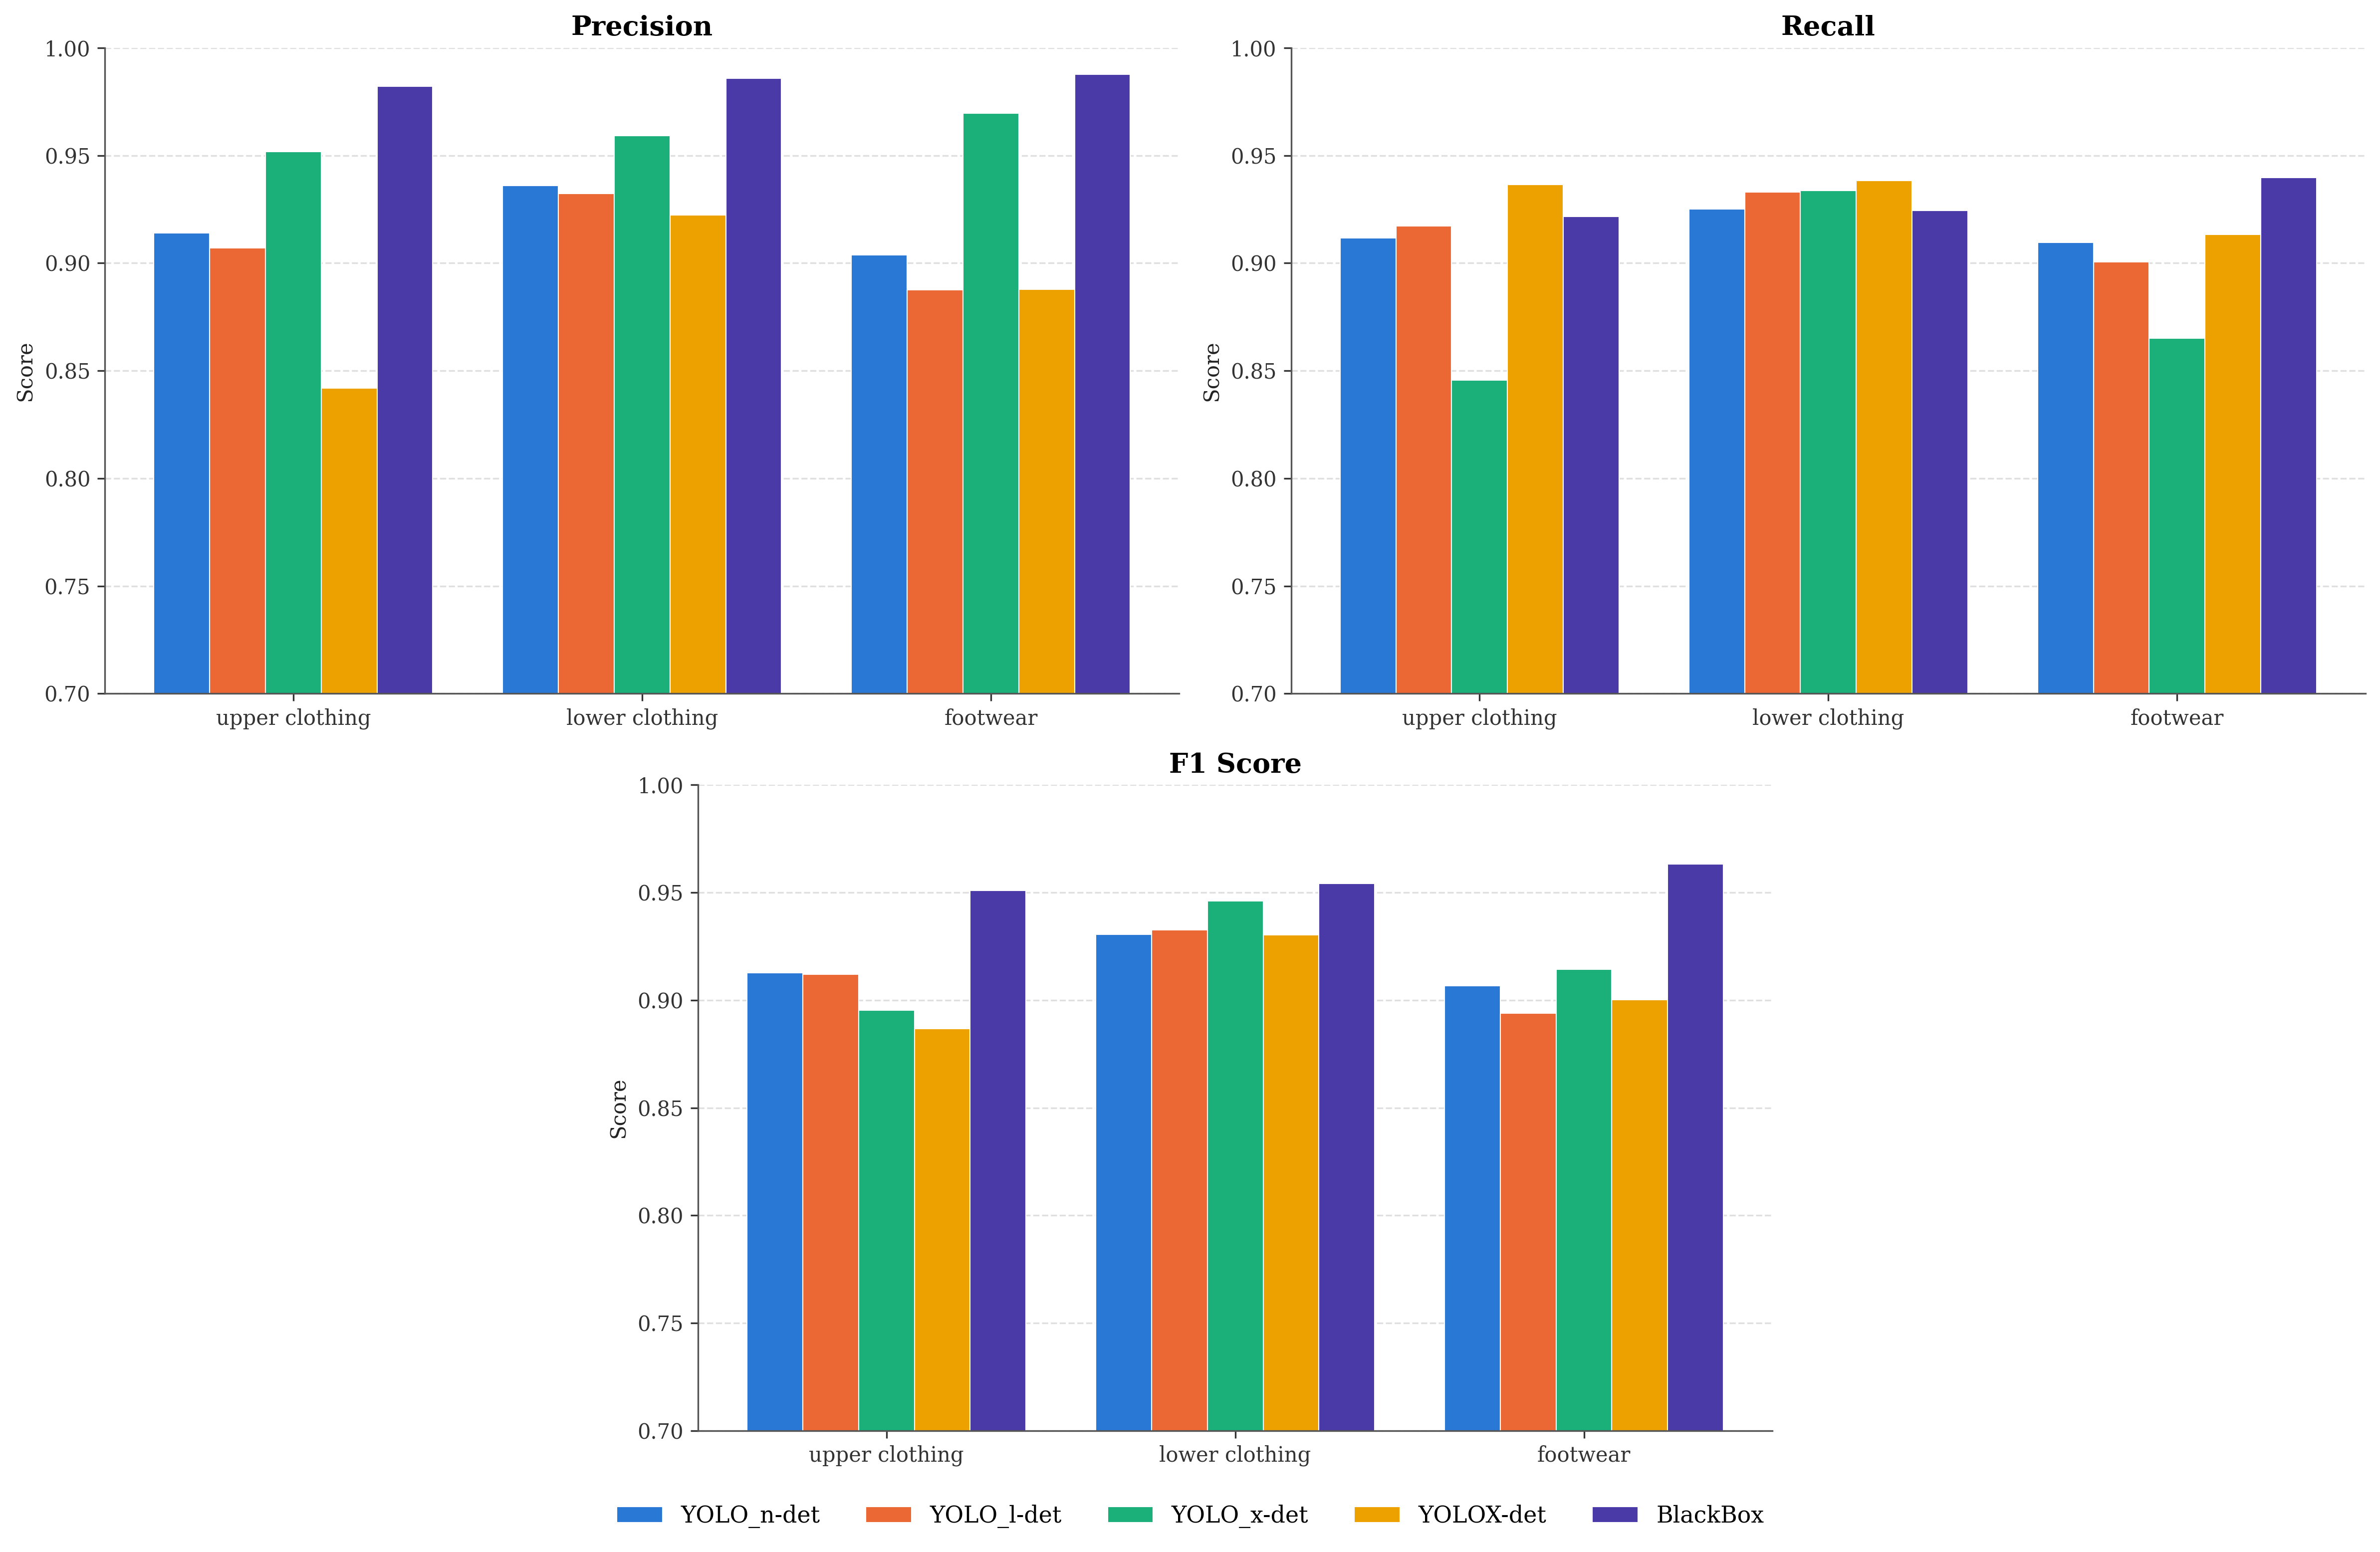
\includegraphics[width=1.2\textwidth]{images/stats/comparison_YOLO_det.png}}
  \label{fig:comparison_YOLO_det}
\end{figure}

\noindent
Come si può osservare, il modello black box mantiene la precision più alta su tutte e tre le classi, con valori vicini a 0.98, e solo YOLO\_x-det riesce ad avvicinarsi a questo risultato, in particolare su \textit{footwear}.
YOLO\_x-det paga però questa precision con una recall sensibilmente più bassa su \textit{upper clothing} e \textit{footwear}, risultando più conservativo: produce poche predizioni errate ma tralascia più oggetti.
YOLOX-det mostra il comportamento opposto, con la recall più alta sulle prime due classi, superiore anche a quella del black box, ma con la precision più bassa, che su \textit{upper clothing} scende a circa 0.84.

\noindent
YOLO\_n-det e YOLO\_l-det si collocano in una posizione intermedia, con precision e recall più bilanciate; da notare che la versione large non supera mai in modo significativo la versione nano.
In termini di F1 score, YOLO\_x-det risulta il più vicino al black box su \textit{lower clothing} e \textit{footwear}, mentre su \textit{upper clothing} viene superato dalle versioni nano e large.

\newpage

\subsection{YOLO segmentation}
Il secondo confronto mette a paragone le varianti di YOLO per la segmentazione, con il miglior modello di detection individuato in precedenza, YOLO\_x-det.

\begin{figure}[htbp]
  \centering
  \makebox[\textwidth][c]{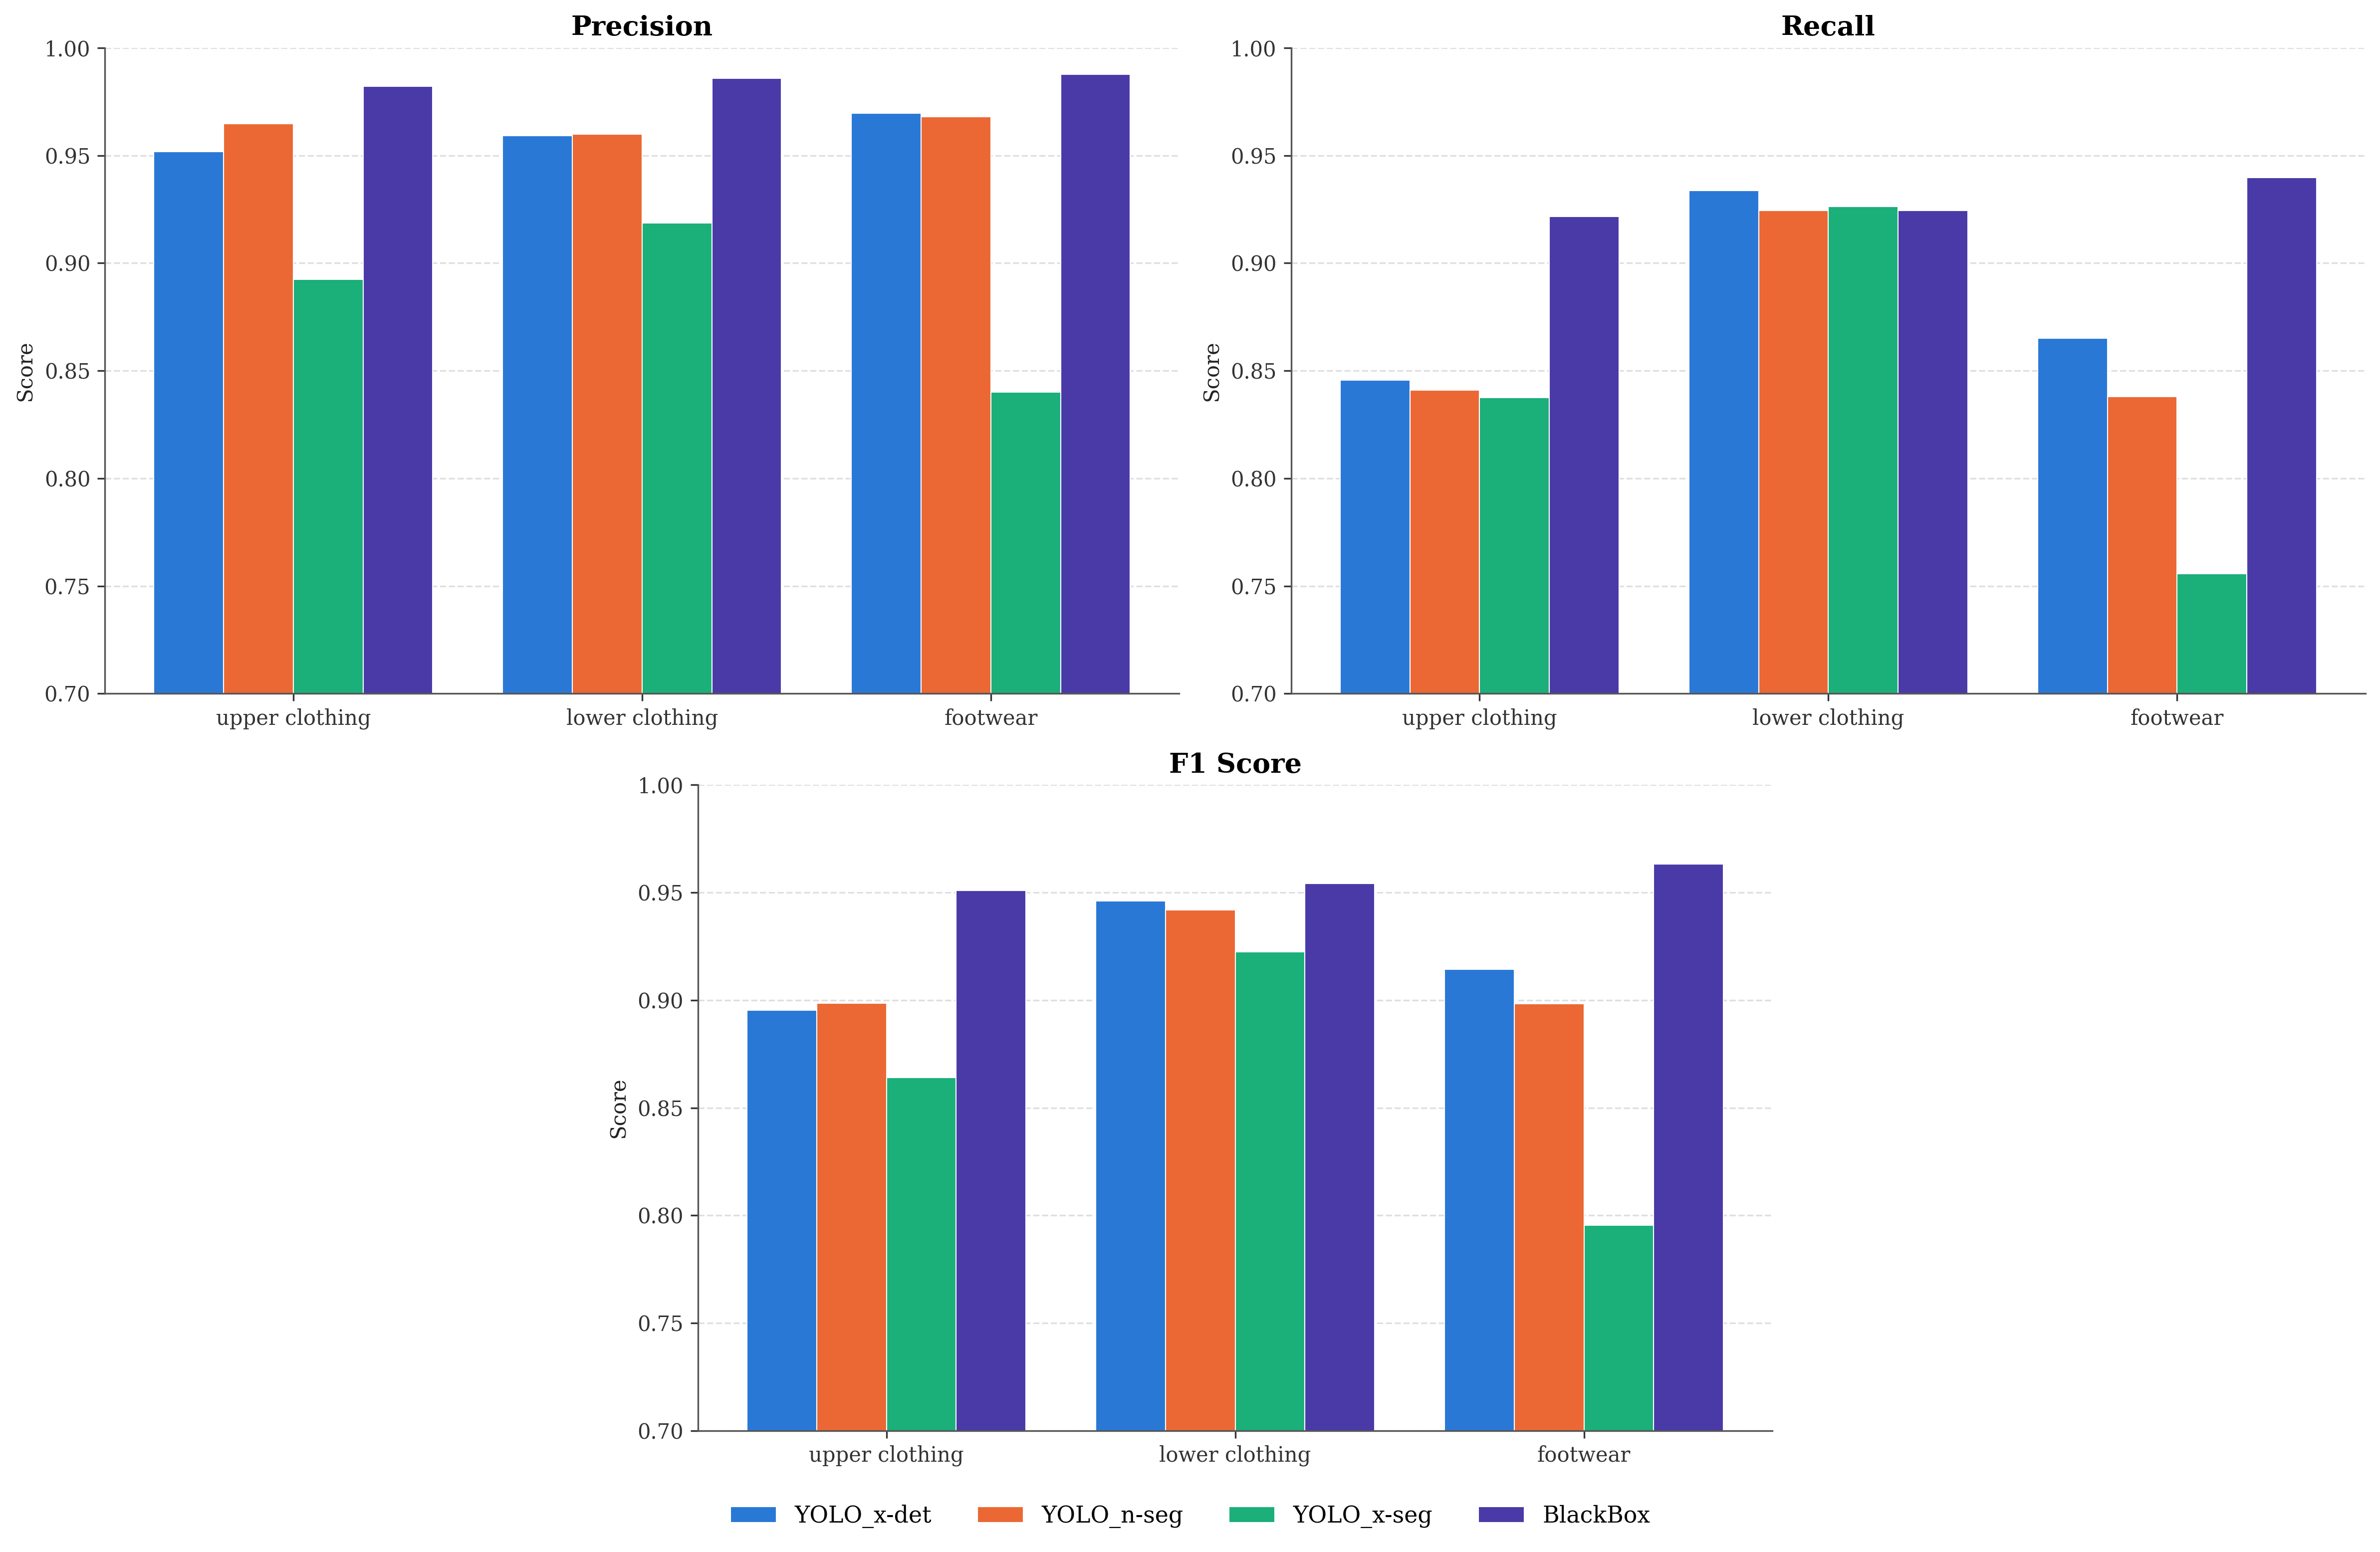
\includegraphics[width=1.2\textwidth]{images/stats/comparison_YOLO_seg.png}}
  \label{fig:comparison_YOLO_seg}
\end{figure}

\noindent
Dal grafico emerge che YOLO\_n-seg ottiene risultati molto simili a YOLO\_x-det: la precision è sostanzialmente la stessa, mentre la recall è di poco inferiore, soprattutto su \textit{footwear}.
Ne deriva un F1 score quasi identico sulle prime due classi e leggermente più basso sulla terza; anche in questo caso, quindi, la versione più piccola del modello si dimostra competitiva.

\noindent
YOLO\_x-seg ha invece prestazioni complessivamente inferiori, in modo evidente su \textit{footwear}, dove la precision si ferma a circa 0.84 e la recall scende intorno a 0.75,
portando l'F1 score sotto 0.80. Le calzature, essendo oggetti piccoli e spesso parzialmente coperti, rappresentano la classe più difficile per questo modello.

\noindent
Tutti e tre i modelli hanno infine una recall su \textit{upper clothing} intorno a 0.84, circa otto punti al di sotto del black box, mentre su \textit{lower clothing} risultano allineati a quest'ultimo.

\newpage

\subsection{SegFormer}
Il terzo confronto riguarda i modelli basati su SegFormer: SegF\_HF e SegF\_StyleMix, confrontati con YOLO\_x-seg.

\begin{figure}[htbp]
  \centering
  \makebox[\textwidth][c]{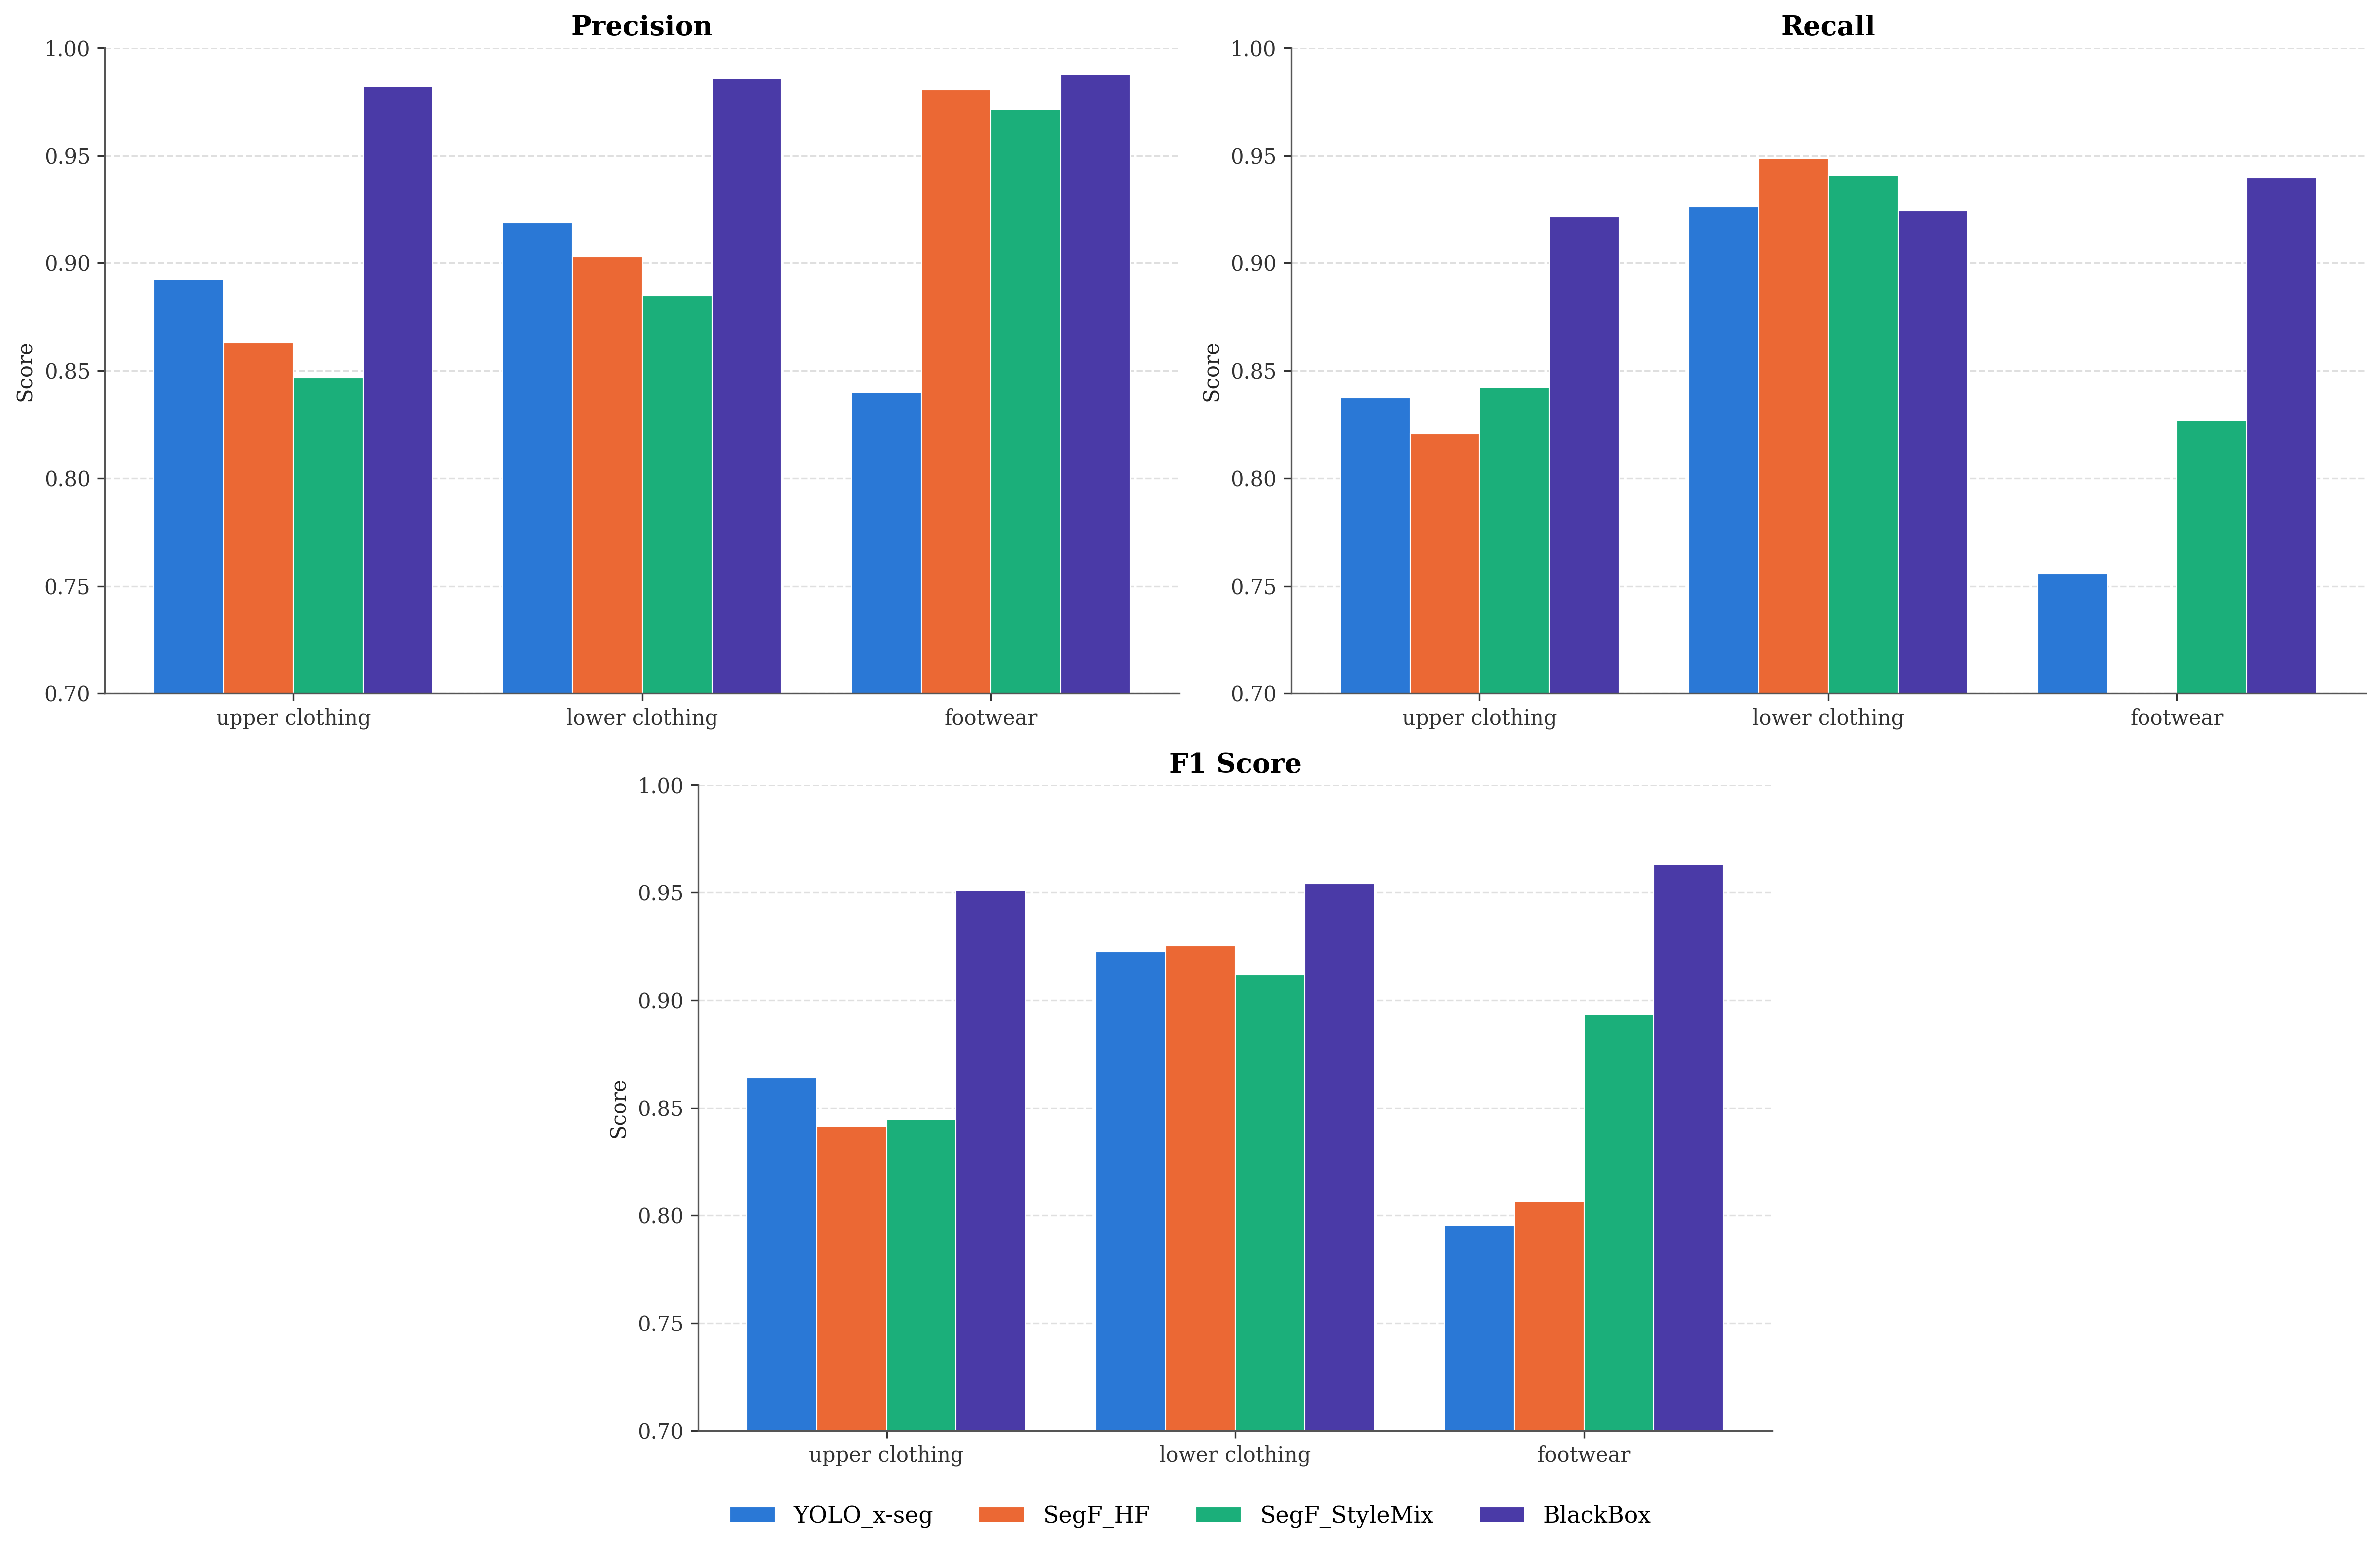
\includegraphics[width=1.2\textwidth]{images/stats/comparison_SegFormer.png}}
  \label{fig:comparison_SegFormer}
\end{figure}

\noindent
In figura si nota come i modelli SegFormer abbiano una precision molto elevata su \textit{footwear}, vicina a quella del black box e nettamente superiore a YOLO\_x-seg.
A questa corrisponde però una recall bassa, che nel caso di SegF\_HF scende al di sotto della scala del grafico: il modello individua con sicurezza le calzature che trova, ma ne tralascia una parte consistente.
SegF\_StyleMix migliora sensibilmente questo aspetto, portando la recall a circa 0.83 e ottenendo su questa classe l'F1 score più alto tra i modelli di segmentazione, pur restando al di sotto del black box.

\noindent
Su \textit{upper clothing} i modelli SegFormer hanno una precision inferiore a YOLO\_x-seg e una recall simile, per cui è quest'ultimo a ottenere l'F1 score migliore.
Su \textit{lower clothing}, invece, raggiungono la recall più alta del grafico, superando anche il black box, ma la precision più bassa mantiene l'F1 score in linea con quello di YOLO\_x-seg.

\newpage

\subsection{GroundingDINO}
Il quarto confronto riguarda i modelli open-vocabulary GroundingDino\_tiny e GroundingDino\_base, confrontati con YOLO\_x-det.

\begin{figure}[htbp]
  \centering
  \makebox[\textwidth][c]{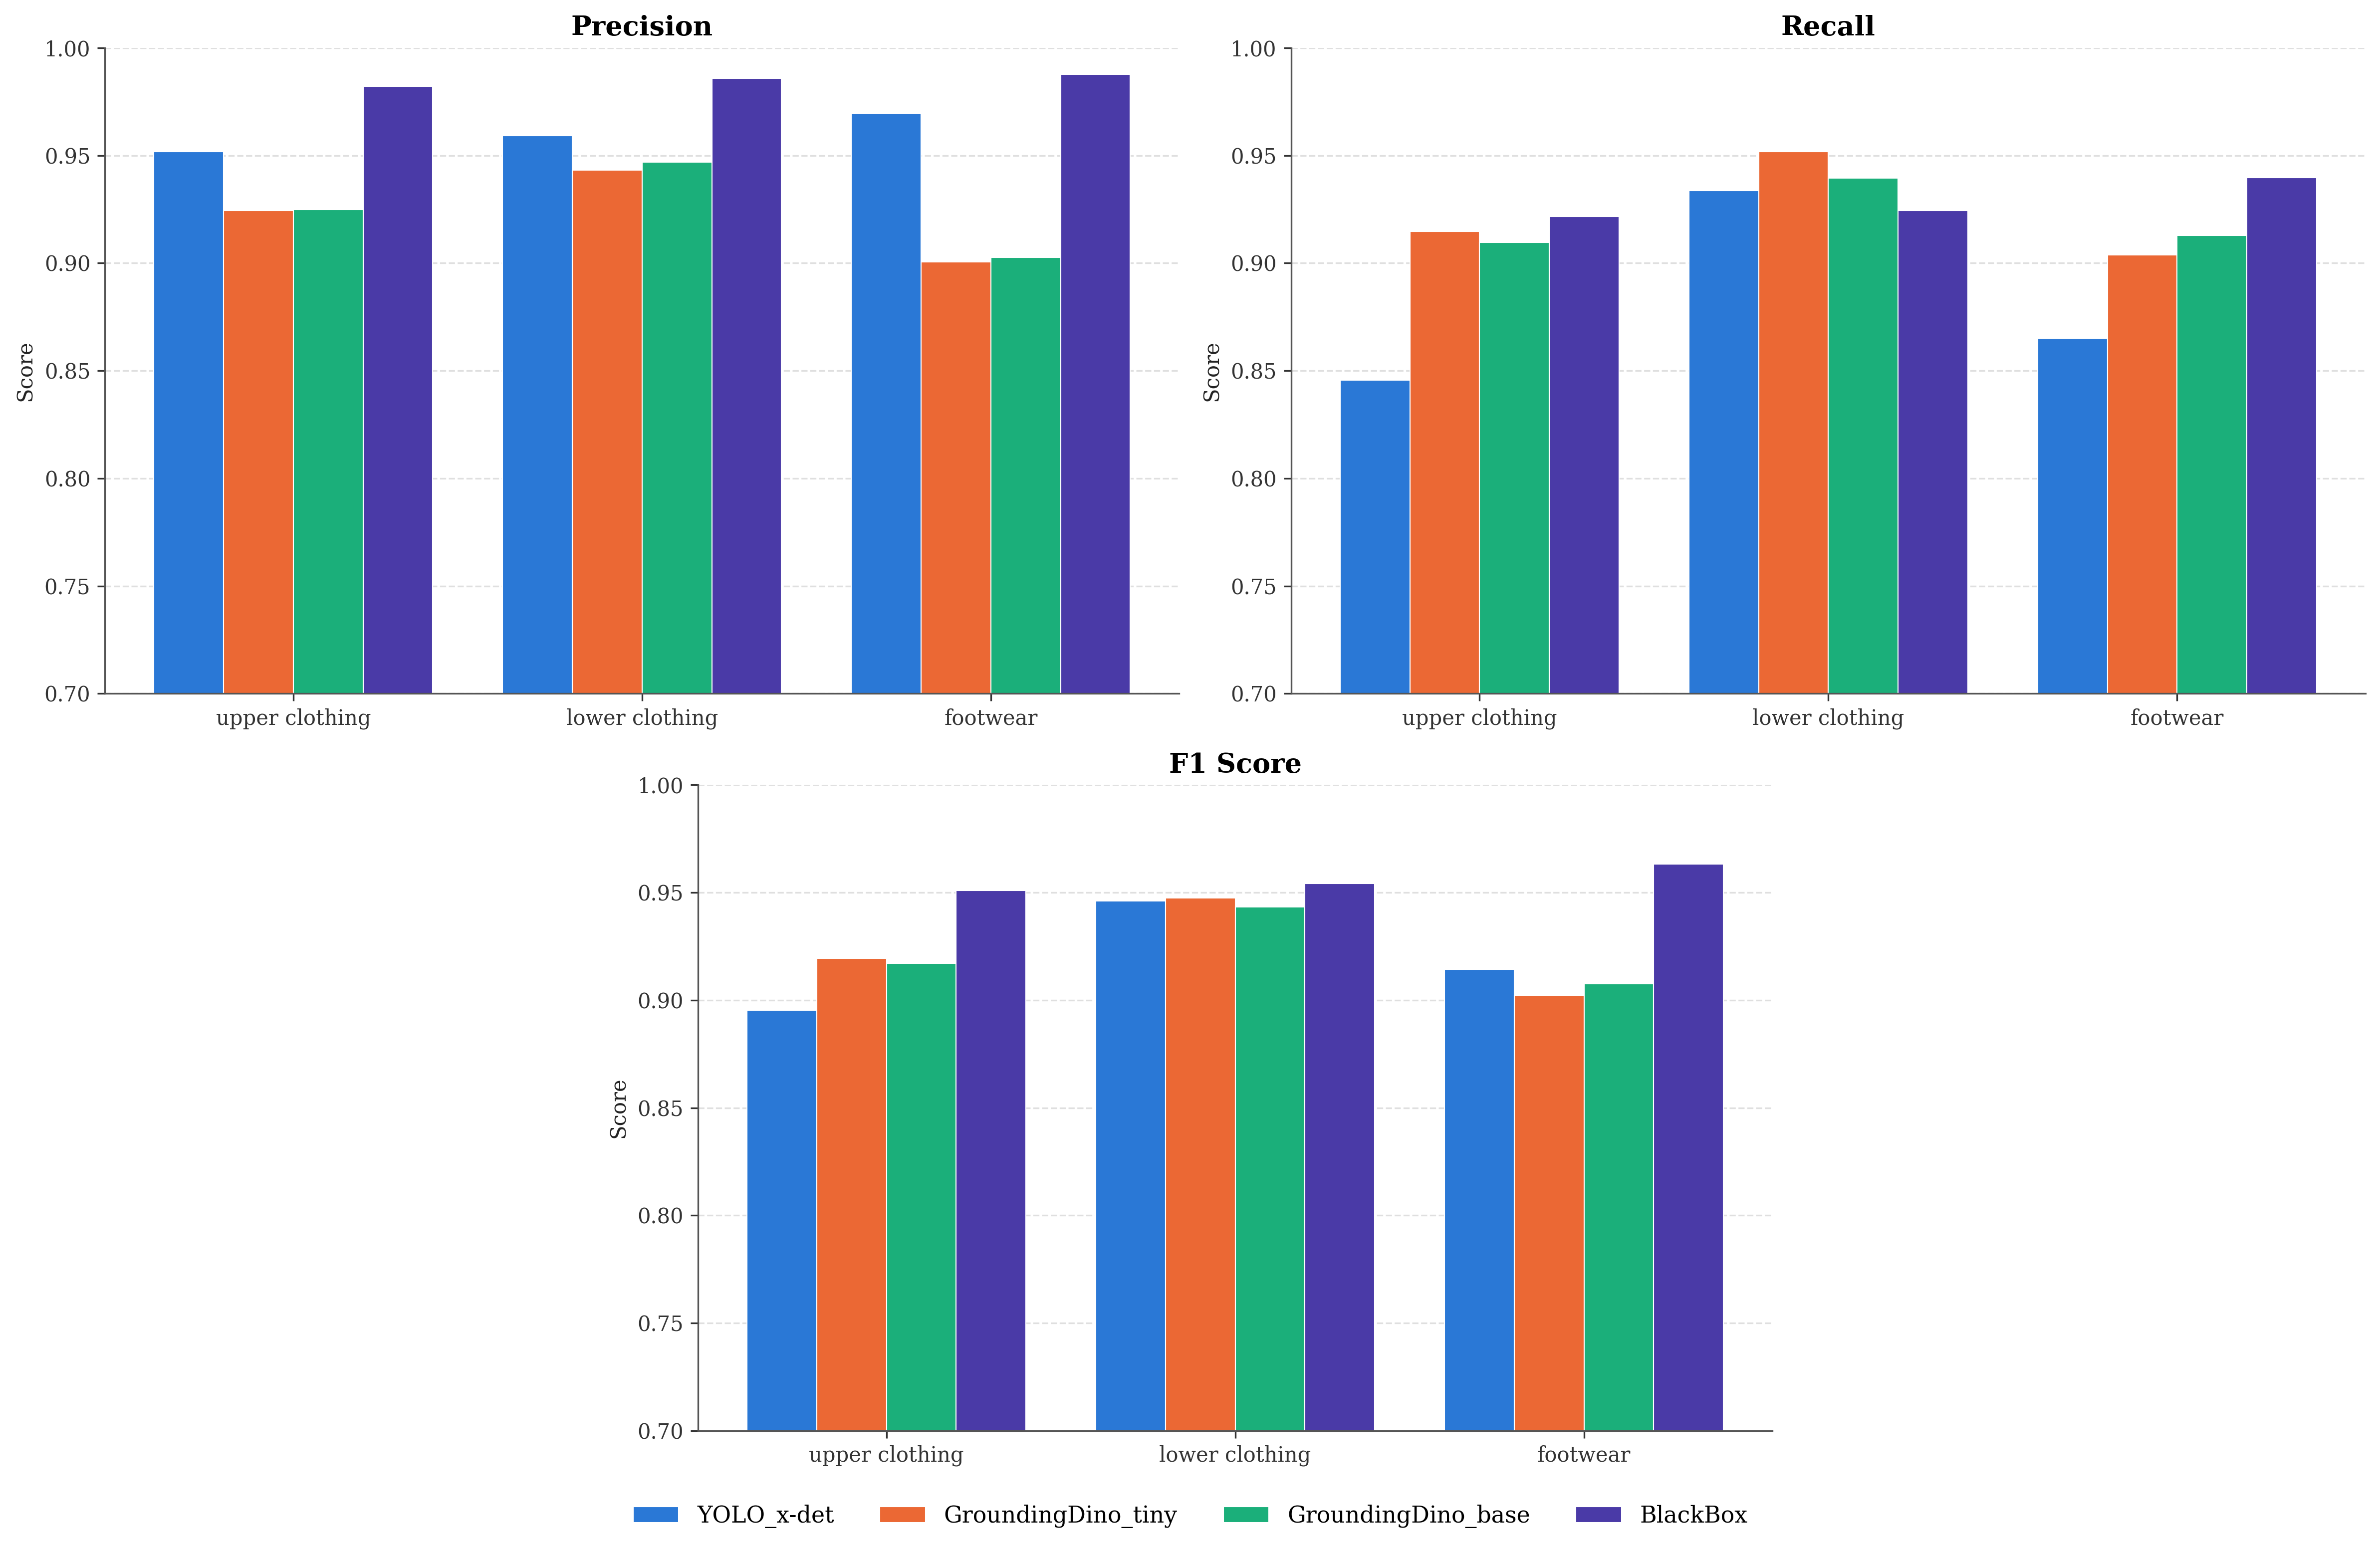
\includegraphics[width=1.2\textwidth]{images/stats/comparison_GroundingDino.png}}
  \label{fig:comparison_GroundingDino}
\end{figure}

\noindent
Come mostrato, entrambe le versioni di GroundingDINO hanno una precision inferiore a YOLO\_x-det su tutte le classi, con un distacco più ampio su \textit{footwear}, dove scendono a circa 0.90 contro 0.97.
In compenso, la recall è più alta su tutte le classi: su \textit{upper clothing} passa da circa 0.85 a 0.91, e su \textit{lower clothing} GroundingDino\_tiny raggiunge circa 0.95, superando anche il black box.

\noindent
Ne risulta un F1 score migliore su \textit{upper clothing}, sostanzialmente equivalente su \textit{lower clothing} e leggermente inferiore su \textit{footwear}, dove il calo di precision non viene compensato del tutto dalla recall.
Le differenze tra la versione tiny e la versione base sono minime, nell'ordine di un punto percentuale o meno: anche in questo caso, un modello più grande non porta vantaggi significativi.

\newpage

\subsection{SAM3}
Infine, abbiamo confrontato SAM3 con i migliori modelli emersi dai confronti precedenti: YOLO\_x-det e SegF\_StyleMix.

\begin{figure}[htbp]
  \centering
  \makebox[\textwidth][c]{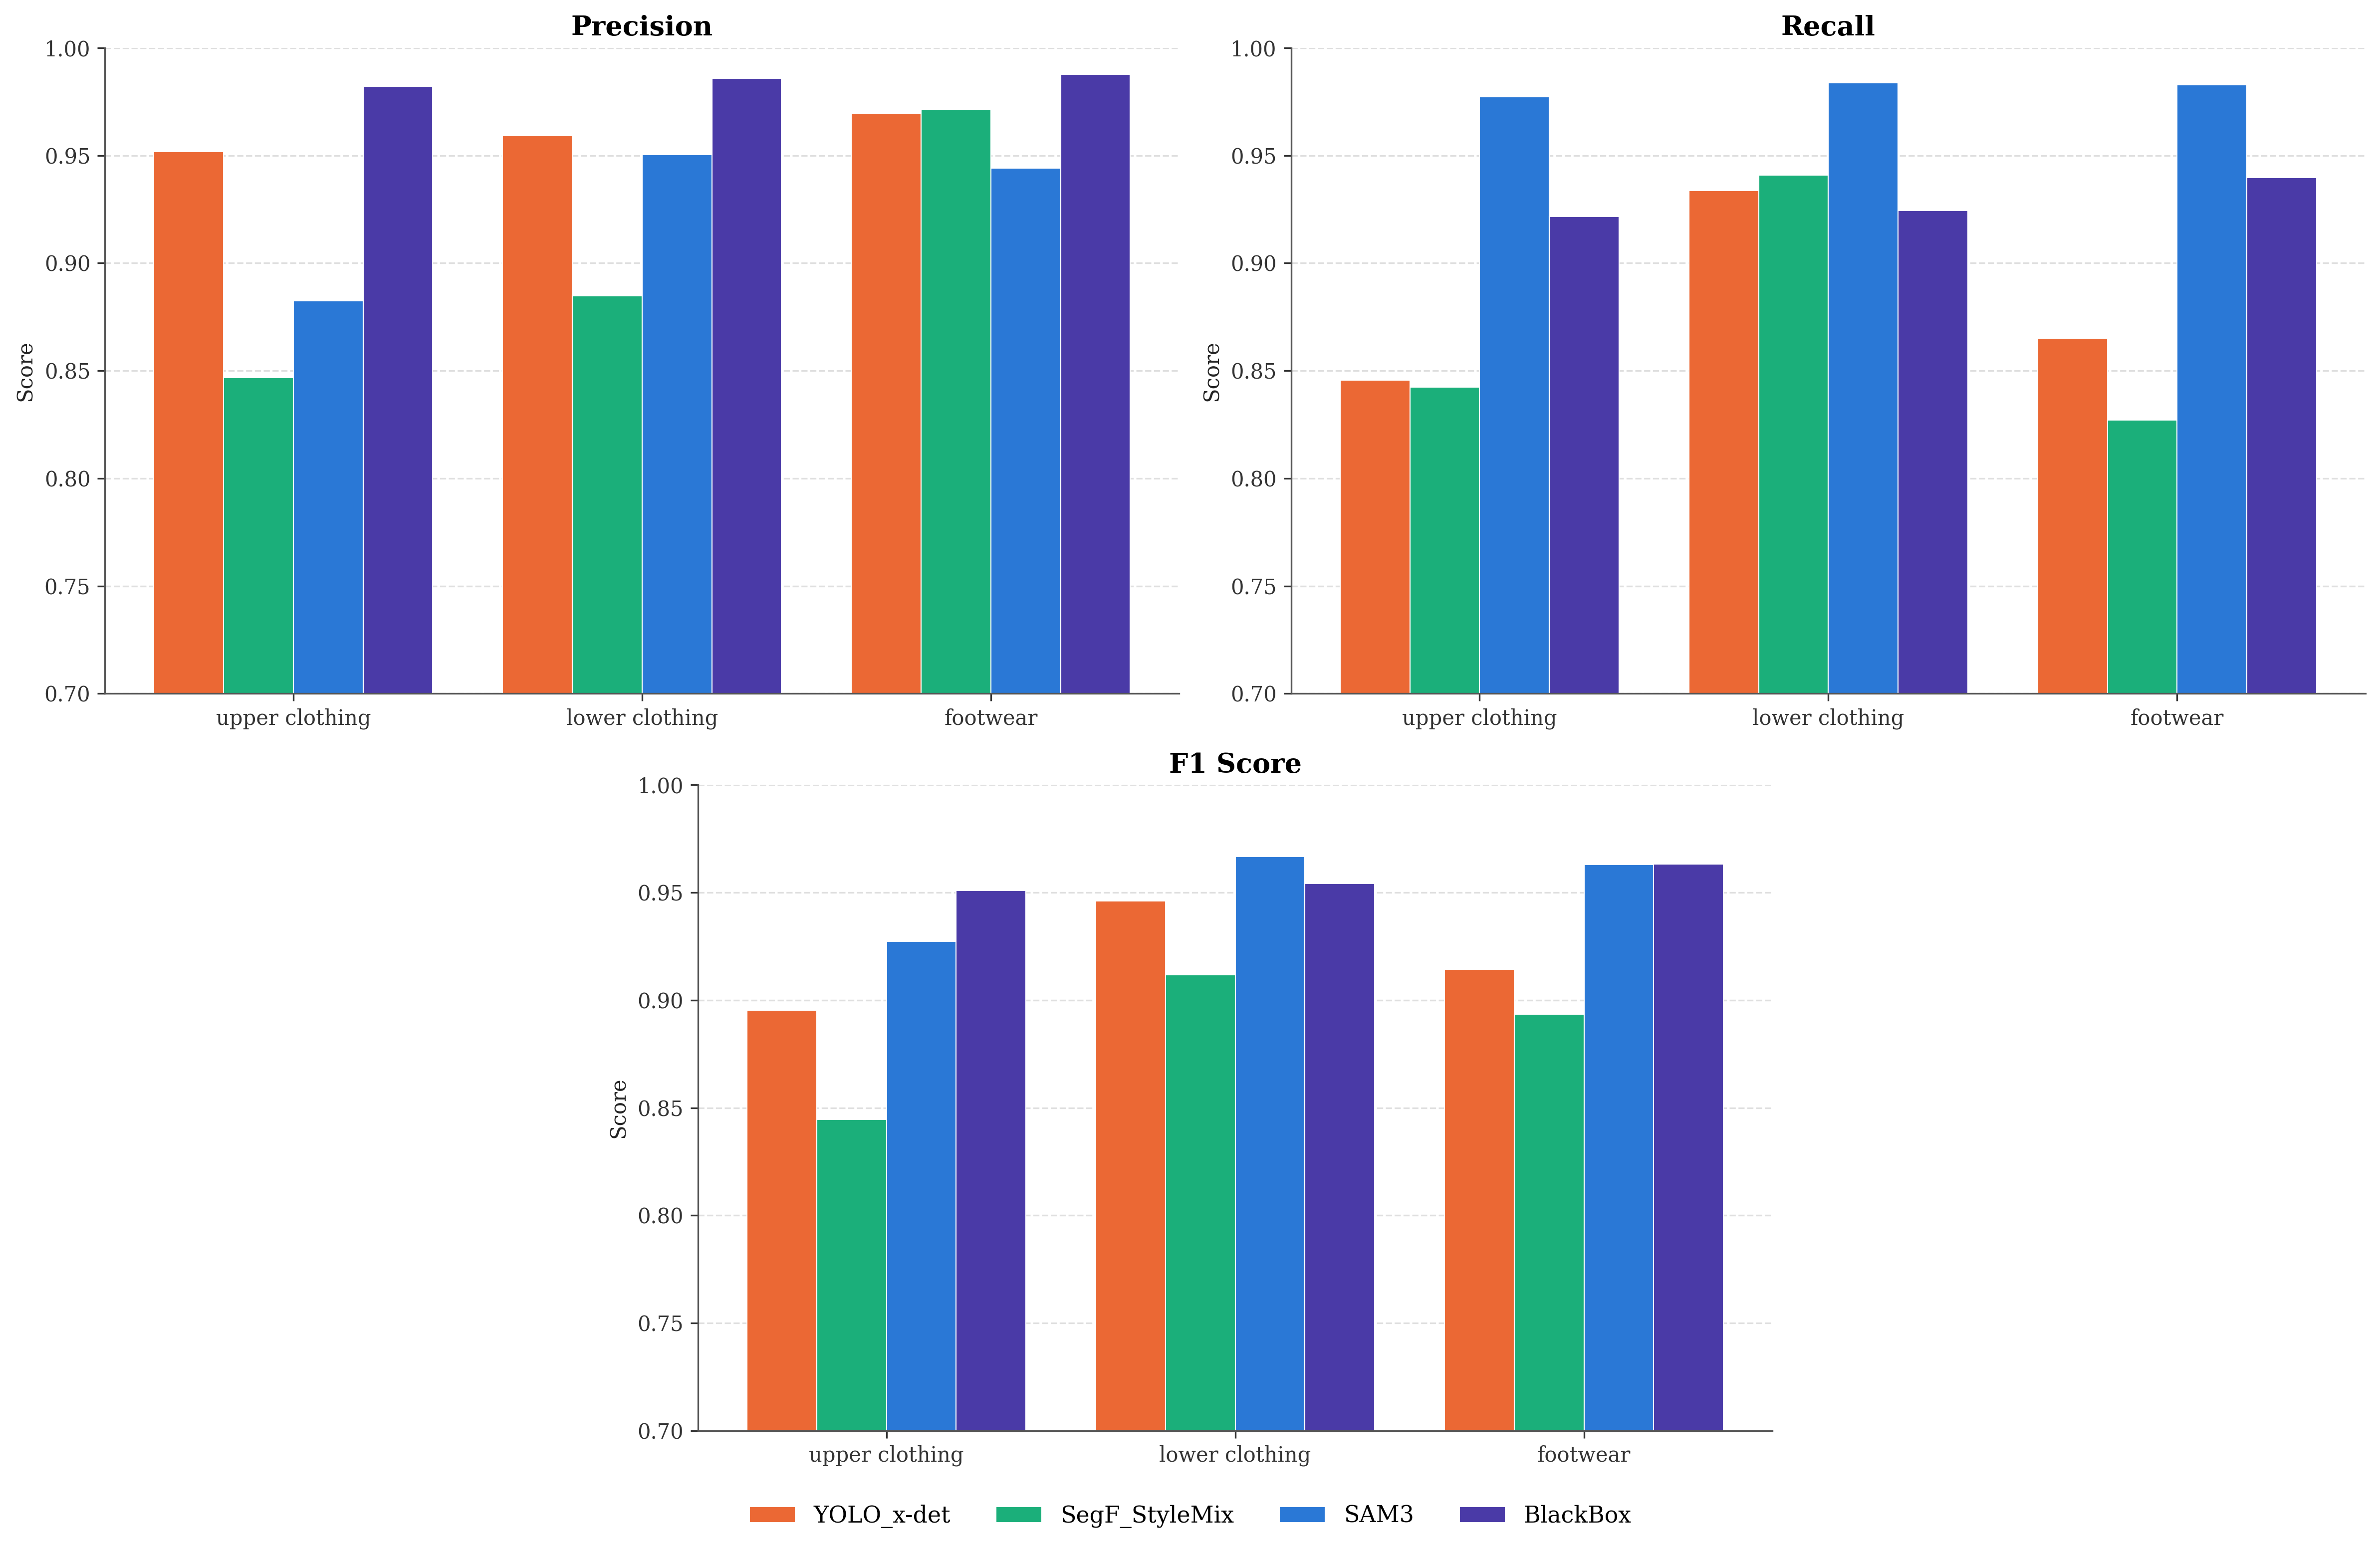
\includegraphics[width=1.2\textwidth]{images/stats/comparison_SAM3_vs_best.png}}
  \label{fig:comparison_SAM3_vs_best}
\end{figure}

\noindent
Qui emerge che SAM3 raggiunge la recall più alta in assoluto, superiore a 0.97 su tutte le classi e quindi anche a quella del black box, che si ferma tra 0.92 e 0.94.
Il vantaggio è particolarmente evidente rispetto a YOLO\_x-det e SegF\_StyleMix su \textit{upper clothing} e \textit{footwear}, dove questi ultimi si fermano intorno a 0.83--0.87.

\noindent
La sua precision resta invece inferiore a quella del black box, con un distacco di circa dieci punti su \textit{upper clothing} e di circa quattro sulle altre due classi.
SAM3 e il black box presentano quindi profili di errore complementari: il primo tende a produrre qualche falso positivo in più, il secondo a tralasciare qualche oggetto.

\noindent
In termini di F1 score, SAM3 supera il black box su \textit{lower clothing}, lo eguaglia su \textit{footwear} e rimane leggermente al di sotto su \textit{upper clothing}.
Ottiene inoltre l'F1 score migliore del confronto su tutte le classi, risultando il modello più vicino al riferimento esterno e l'unico in grado di raggiungerne o superarne le prestazioni su almeno una classe.

\newpage

\section{Dai modelli al sistema}

Il percorso seguito fin qui ha avuto un obiettivo preciso, cioè capire quale fosse lo strumento più adatto a riconoscere i capi d'abbigliamento all'interno di una fotografia.
Dopo aver introdotto i concetti alla base delle reti neurali e del loro addestramento, abbiamo analizzato e addestrato modelli di natura molto diversa, i quali per poterli confrontare in modo equo
abbiamo costruito una ground truth verificata a mano e un protocollo di valutazione comune, che ha permesso di misurarli tutti con lo stesso metro e di metterli a confronto con un modello esterno di riferimento.

Il risultato di questo confronto è stato netto. SAM3 si è rivelato il modello con la recall più alta, in grado di individuare la quasi totalità dei capi presenti nelle immagini,
e l'unico a raggiungere o superare il modello "black box" in termini di F1 score su almeno una classe.
A questo si aggiunge un vantaggio che le metriche non misurano direttamente, SAM3 non richiede alcun addestramento sul nostro dominio, perché viene interrogato in linguaggio naturale,
e può quindi cercare qualunque tipo di capo semplicemente cambiando il prompt testuale.

Riconoscere un capo, però, non è di per sé un risultato utile per l'utente finale. Un modello di segmentazione restituisce maschere e riquadri, cioè informazioni che descrivono una singola immagine,
ma non ci dice nulla sui rapporti tra i prodotti di un catalogo, quali capi vengono indossati insieme, quali stili si abbinano, quale articolo potrebbe completare un outfit.
Per rispondere a domande di questo tipo serve una struttura capace di raccogliere ciò che il modello osserva nelle singole fotografie e di trasformarlo in conoscenza organizzata e interrogabile.

Le fotografie indossate di un catalogo contengono un'informazione implicita molto preziosa: ogni immagine mostra un abbinamento reale, scelto da chi ha curato il catalogo.
Utilizzando SAM3 per isolare i singoli capi presenti in ciascuna fotografia, e riconducendo poi ogni capo all'articolo corrispondente tramite una ricerca per somiglianza visiva, è possibile trasformare queste co-occorrenze in un grafo,
in cui i prodotti sono i nodi e gli abbinamenti osservati sono le relazioni tra di essi.

Il lavoro svolto nei capitoli precedenti non rappresenta quindi un fine a sé stante, ma la base su cui poggia un sistema concreto, cioè l'analisi dei modelli ha permesso di scegliere in modo motivato il componente più affidabile,
e il protocollo di valutazione ha dato una misura oggettiva di quanto ci si possa fidare delle sue predizioni.
Nel prossimo capitolo vedremo come questo componente venga integrato in un'architettura GraphRAG, che affianca un database vettoriale per la ricerca per somiglianza e un database a grafo per la gestione delle relazioni,
dando vita a un sistema in grado di rappresentare e interrogare gli abbinamenti tra i prodotti del catalogo.

\newpage
